% !TeX root = ../main.tex

\chapter{绪论}
\label{ch1}

\section{引言}

凝聚态物理的任务是研究各种材料的性质。在看似错综复杂的不同系统中,Landau提出了试图统一凝聚态物理的基本原理\cite{Landau:480039}:不同的物相由不同的局域序参量刻画,不同的序参量对应着不同的对称性破缺,而相变就是对称性破缺模式的变化。利用群论的语言,Ginzberg和Landau发展了相和相变的标准理论\cite{Landau:486430}。然而,随着二维Berezinskii–Kosterlitz–Thouless相变理论\cite{Kosterlitz1973}的提出和强磁场下二维电子气中的整数\cite{Klitzing1980}和分数\cite{Tsui1982}量子霍尔效应的发现,人们逐渐意识到存在超越Landau标准理论的新物态,现被称为拓扑物态。与对称破缺有序相不同,拓扑物态无法只用局域序参量刻画,还必须利用到数学上的拓扑不变量的概念。拓扑不变量刻画的是系统的全局性质,其最重要的特征就是它只能取离散的数值,因而在系统参数连续变化时可以保持不变。物理地说,拓扑物态有非常稳定的物理性质,例如在最早的二维整数量子霍尔效应中,半经典模型下随磁场线性增加的霍尔电阻在低温下呈现出一系列平台,这些平台对样品的几何是如此不敏感,以至于可以被用来标定精细结构常数。拓扑物态的另一个重要特性就是所谓的体-边对应,即拓扑非平庸的体拓扑对应于边界上存在拓扑保护的零能模。整数霍尔效应的霍尔平台就是由于边界上存在的无能隙手征模式,这些无法被向后散射的态是理想的导电通道。

1988年,Haldane首先指出整数量子霍尔效应的本质是时间反演对称性被破坏,而磁场不是必须的\cite{Haldane1988},据此提出的量子反常霍尔效应已在拥有磁性参杂的拓扑绝缘体\cite{Chang2013}以及冷原子体系\cite{Jotzu2014}实现。2005年,美国的两个小组又理论预言了二维量子自旋Hall效应\cite{Kane2005,Bernevig2006a},他们指出为了实现量子Hall效应而破坏时间反演对称性也不是必须的。相反,由于有时间反演对称性,无能隙边界态总是成对出现,沿着相反方向传播。很快,量子自旋Hall效应在半导体量子阱HgTe/CdTe中被证实\cite{Bernevig2006}。自此,拓扑能带理论的研究井喷式发展:二维量子自旋Hall效应很快被推广到三维,产生了三维拓扑绝缘体的概念\cite{Moore2007,Fu2007a,Roy2009},这些三维绝缘体的表面是具有奇数个Dirac锥的金属态,很快也被实验证实\cite{Hsieh2008}。由于费米型BdG哈密顿量和自由哈密顿量有相同的形式,拓扑绝缘体的概念也被直接推广到拓扑超导体。例如在一维p-波超导体中,Kitaev指出拓扑相的超导体两端分别存在一个稳定的Majorana零能模\cite{Kitaev2001}。这些分隔很远的Majorana零模可以非局域地存储量子比特的信息,从而对抗环境噪声影响。另外它们还有非阿贝尔统计\cite{Ivanov2001},当存在多个Majorana零模时,对它们进行编织操作等效于对量子比特做逻辑门操作,因而可用于拓扑量子计算\cite{Pachos2014}。
随着拓扑能带理论研究的深入,人们开始把各种可能的拓扑绝缘体和拓扑超导体进行分类。早期的分类是根据哈密顿量是否具有非空间(內禀)对称性:时间反演对称性、粒子-空穴对称性和手性对称性 \cite{Altland1997,Zirnbauer2018}。得到的所谓十重拓扑分类显示,在任意维度,十个对称类中有五个对称类是存在非平凡拓扑相的。随后又发现当有额外的空间对称性时,体拓扑数有简化的表达式 \cite{Fu2007},甚至拓扑分类自身都被扩展了 \cite{Fu2011}。这些包含空间对称性的拓扑物态最终导致了晶体拓扑绝缘/超导体的概念\cite{Ando2015},随后还建立了拓扑材料在线数据库\cite{vergniory2019complete,zhang2019catalogue,tang2019comprehensive}。在晶体拓扑绝缘/超导体这一大类里,最近又衍生出所谓的高阶拓扑绝缘/超导体\cite{Benalcazar2017,Langbehn2017,Benalcazar2017a,Schindler2018}。另外,一些动力学\cite{Chang2018,Yang2018,Gong2018,Qiu2018}、开放量子系统 \cite{Shen2018,Kawabata2018,Kawabata2019,Song2019},非厄米物理系统\cite{Yao2018a,Yao2018,Xiao2020}的拓扑性质也开始被广泛研究。

2005年,Haldane和Raghu \cite{Raghu2008,Haldane2008}又指出,拓扑能带理论(即带有非平庸拓扑数的能带结构决定并保护了边界态的存在)不是与费米子绑定的,其本质上是一种波效应;利用非倒易的(法拉第效应)介质,他们提出在光学系统中实现量子霍尔边界态的对应。自此,在其他物理系统中实现或利用拓扑能带理论的工作不断涌现,例如磁性晶体 \cite{Shindou2013,Chisnell2015,Kondo2019}, 光子晶体 \cite{Wang2008,Rechtsman2013,Peano2016}, 声子晶体 \cite{Fleury2014,SafaviNaeini2014,Peano2015} 甚至大气物理\cite{Delplace2017}。

本文关注的是光晶格中相互作用超冷玻色子在进入有序相后其集体激发的能带拓扑结构。近年来随着量子模拟调控技术的发展,各种拓扑能带已经在冷原子气体实验中实现\cite{Goldman2016,Cooper2019}。当在这些能带中放入玻色子时,极低温下一般仍有玻色爱因斯坦凝聚现象。事实上,已有一些工作表明这些玻色爱因斯坦凝聚体的集体激发的能带存在拓扑结构 \cite{Furukawa2015,Xu2016,Liberto2016}。但是之前工作都是关注于最简单的拓扑能带(属于破坏时间反演对称性的A类),而且都是考虑在弱相互作用极限。本文中我们主要研究了两个问题:
\begin{itemize}
    \item 对于十重分类里其他的拓扑相,能否在玻色超流体的Bogoliubov激发谱中找到对应。作为一个最经典的例子,我们找到了二维时间反演对称拓扑绝缘体(AII类)所对应的能带拓扑在玻色超流体激发谱中的对应。
    \item 在玻色超流的强相互作用区间,其低能激发的能带拓扑又有什么特性。特别地,一个非常有趣的问题是:在超流-Mott绝缘相变临界点附近是否存在涌现的拓扑Higgs振幅模。通过考察一个具体模型,我们对此问题给出了肯定回答。
\end{itemize}
在本章的剩下部分,我们首先讨论了规范理论中的拓扑,然后具体回顾了传统(自由费米子的)拓扑能带理论。

%%%%%%%%%%%%%%%%%%%%%%%%%%%%%%%%%%%%%%%%%%%%%%%%%%%%%%%%%%%%%%%%%%
\section{规范理论中的拓扑}
%%%%%%%%%%%%%%%%%%%%%%%%%%%%%%%%%%%%%%%%%%%%%%%%%%%%%%%%%%%%%%%%%%
我们最早接触到物理学中的拓扑可能是在电磁学中:注意到高斯定理和安培定理涉及的面积分和线积分在面、线的连续变形下是不变的。这些积分实际上定义了拓扑不变量。这一节,我们讨论规范理论中的拓扑。一方面它展示了拓扑学在物理中的应用;更重要的是,这些概念在拓扑能带理论(下一节讨论)中都有直接对应。

\subsection{一个例子:磁荷量子化的拓扑起源}
%%%%%%%%%%%%%%%%%%%%%%%%%%%%%%%%%%%%%%%%%%%%%%%%%%%%%%%%%%%%%%%%%%
Maxwell方程统一了电和磁,但它是非对称的。Dirac提出可以通过定义磁单极子来使电磁理论对称\cite{dirac1931}。假设有一个强度为$g$的磁单极子在$\vb r = 0$处,
\begin{equation}
  \ddiv \vb B = 4\pi g \delta^3(\vb r)
\end{equation}
那么它对应的解是
\begin{equation}
  \vb B = g \frac{\vb r}{r^3}.
\end{equation}
所以对于一个包围原点的球$V$,穿过其表明$\partial V$的总磁通是
\begin{equation}
  \Phi = \oint_{\partial V} \vb B \cdot \dif \vb S = 4\pi g.\label{phib}
\end{equation}
注意到如下定义的矢势$\an$
\begin{equation}
  \an = \frac{-g y}{r(r+z)}\vu{e}_x + \frac{g x}{r(r+z)}\vu{e}_y=\frac{g(1-\cos \theta}{r\sin \theta}\vu{e}_\phi
\end{equation}
满足
\begin{equation}
  \ccurl \an = g \frac{\vb r}{r^3} + 4 \pi g \delta(x)\delta(y)\theta(-z).
\end{equation}
即除了在负$z$-轴(被称作Dirac弦)是奇异的,我们有$\ccurl \an = \vb B$。
类似地,我们可以选取另一个矢势,
\begin{equation}
  \as = \frac{g y}{r(r-z)} \vu{e}_x + \frac{-g x}{r(r-z)}\vu{e}_y = -\frac{g(1+\cos\theta)}{r\sin \theta} \vu{e}_\phi.
\end{equation}
这时对应的Dirac弦在正$z$-轴。
无论怎么选取规范,Dirac弦始终存在;毕竟如果由$\vb B = \ccurl \vb A$给出的矢势是良好定义的,由Stokes定理我们有
\begin{equation}
  \Phi = \oint_{\partial V} \vb B \cdot \dif \vb S = \oint_{\partial V} \ccurl \vb A\cdot \dif \vb S = \int_V \ddiv (\ccurl \vb A) \dif V= 0.
\end{equation}
这与式\eqref{phib}矛盾。

Dirac的磁单极子模型中矢势是有奇异的,Wu和Yang注意到我们可以利用两个矢势来描述一个磁单极子从而避免奇异性\cite{wu1976}。例如,我们在北半球用$\an$、在南半球用$\as$来将磁单极子包裹住。这样定义的矢势处处给出$\vb B= g \vb r / r^3$。在该球的赤道上,$\an$和$\as$由一个规范变换联系,
\begin{equation}
  \ggrad \Lambda = \an - \as = \frac{2g}{r \sin \theta} \vu{e}_\phi = \ggrad (2g\phi)\quad \Longrightarrow \quad \Lambda = 2g \phi.
\end{equation}
注意$\Lambda$在$\theta =0$和$\theta = \pi$是无良好定义的,不过我们只在$\theta = \pi/2$进行这个规范变换,从而避免了这个奇异性。在这样定义的矢势下,我们重新计算总磁通
\begin{equation}
  \Phi = \oint_{\partial V} \ccurl \vb A \cdot \dif \vb S = \int_{U_\text{N}} \ccurl \an \cdot \dif \vb S + \int_{U_\text{S}} \ccurl \an \cdot \dif \vb S
\end{equation}
其中$U_{\text N}$和$U_{\text S}$分别是北半球和南半球。由于在对应区域内矢势是良好定义的,利用Stokes定理有,
\begin{equation}
  \Phi = \oint_{\partial U_{\text N}} \an\cdot \dif \vb \ell + \oint_{\partial U_{\text S}} \as \cdot \dif \vb \ell 
  =\oint_{\partial U_\tn} (\an -\as) \cdot \dif \vb \ell
  = \oint_{\partial U_{\text N}}\ggrad (2g\phi)\cdot \dif \vb \ell = 4g \pi
\end{equation}
这与式\eqref{phib}吻合。

考虑一个电荷为$e$质量为$m$的电子在一个固定的磁单极子周围运动,其薛定谔方程为
\begin{equation}
  \frac{1}{2m}\pqty{\vb p - \frac{e}{c}\vb A}^2\psi(\vb r) = E\psi(\vb r).
\end{equation}
容易证明在一个规范变换$\vb A \rightarrow \vb A + \ggrad \Lambda$下,波函数的变换是$\psi \rightarrow \eu^{\iu e \Lambda/\hbar c} \psi$。假设$\psi^{\tn}$和$\psi^{\ts}$分别是电子在$U_{\tn}$和$U_{\ts}$上对应的波函数,那么它们由如下联系
\begin{equation}
  \psi^{\ts} (\vb r) = \eu^{\frac{-\iu e \Lambda}{\hbar c}} \psi^{\tn} (\vb r).
\end{equation}
由于单值性,电子波函数在绕赤道一圈后必须回到自己,所以上式暗示
\begin{equation}
  \frac{2e g}{\hbar c} = N \in \mathbb Z.
\end{equation}
这即是Dirac量子化条件。这里的整数$N$是缠绕数,对应于同伦群$\pi_1[\mathrm{U}(1)]=\mathbb Z$,即当$\phi$绕一圈时(从$0$到$2\pi$),$\eu^{\iu e \Lambda/\hbar c}$覆盖规范群$\mathrm{U}(1)$的次数。这正是Dirac磁荷量子化的拓扑来源。实际上这个讨论可以直接推广到非阿贝尔规范场,例如把此处的$\mathrm{U}(1)$阿贝尔规范场换成$\mathrm{SO}(3)$非阿贝尔规范场,我们有$\pi_1[SO(3)]=\mathbb Z_2$,这时磁荷和反磁荷是相同的。

\subsection{阿贝尔规范理论}
%%%%%%%%%%%%%%%%%%%%%%%%%%%%%%%%%%%%%%%%%%%%%%%%%%%%%%%%%%%%%%%%%%
\subsubsection{微分形式表述}
%%%%%%%%%%%%%%%%%%%%%%%%%%%%%%%%%%%%%%%%%%%%%%%%%%%%%%%%%%%%%%%%%%
考虑一个定义在流形$X$,局域坐标为$x^i$,$i=1,\dots,d$,上的阿贝尔规范理论。规范势被定义成是一个协变的一阶张量,即在坐标变换$x^i \rightarrow x^{\prime i}$下,(以后我们假设Einstein求和规则)
\begin{equation}
  a_i \rightarrow a_i' = \frac{\partial x^j}{\partial x^{\prime i}} a_j.\label{adef}
\end{equation}
这个条件使规范协变导数$\partial_i \phi -ia_j \phi$在坐标变换下和$\partial_i \phi$有一样的变换。因此规范势分量可以被组合成一个微分1-形式
\begin{equation}
  a = a_i \dif x^i.
\end{equation}
场$\phi$的协变微分也是一个1-形式$\dif \phi - ia \phi$。注意1-形式$a$是坐标不变的,这由式\eqref{adef}直接得到
\begin{equation}
  a_i \dif x^i = a_i' \dif x^{\prime i}.
\end{equation}
场张量的分量可以被组成一个2形式的场强
\begin{equation}
  f= \dif a = \frac{1}{2} (\partial_i a_j - \partial_j a_i) \dif x^i \wedge \dif x^j,
\end{equation}
即$a$的外微分。注意到它也是坐标不变的。注意外微分的两个基本性质,(i)Leibniz规则:如果$u$是一个$r$-形式,则有$\dif(u\wedge v)= \dif u \wedge v+ (-1)^r u \wedge \dif v$;(ii)$d^2=0$。后则暗示$f$是闭的,即(其中第一个等号是右边等于零给出Bianchi等式)
\begin{equation}
  \dif f = f\wedge a-a \wedge f =  \dif (\dif a) = 0.\label{dfzero}
\end{equation}
由此可得$f$在规范变换
\begin{equation}
  a\rightarrow a+\dif \alpha,
\end{equation}
下是不变的
\begin{equation}
  \dif (a+\dif \alpha) = \dif a + \dif (\dif \alpha) = \dif a.
\end{equation}

Maxwell电磁理论是一个阿贝尔规范理论,其对应的规范群是$\mathrm{U}(1)$。回忆Maxwell方程
\begin{subequations}
    \begin{align}
        \ddiv \vb B &= 0 , \quad \frac{\partial \vb B}{\partial t} + \ccurl \vb E = 0,\label{me1} \\
        \ddiv \vb E &= \rho , \quad \frac{\partial \vb E}{\partial t} - \ccurl \vb B = -\vb j.\label{me2}
    \end{align}
\end{subequations}
我们定义规范势$A_\mu = (\phi,\vb A)=-\iu a_\mu$(注意电磁理论里的矢势和上述矢势相差一个虚数$\iu$),则有
\begin{equation}
  \vb B = \ccurl \vb A,\quad \vb E = \frac{\partial \vb A}{\partial t} - \ggrad \phi.
\end{equation}
电磁场张量是$F_{\mu\nu}=\partial_\mu A_\nu -\partial_\nu A_\mu =-\iu f_{\mu\nu}$,即$E_i = F_{i0}$,$B_i=\frac{1}{2}\epsilon_{ijk}F_{jk}$,或者写成矩阵形式,
\begin{equation}
  F_{\mu\nu} = \begin{bmatrix}
      0 & -E_x & -E_y & -E_z \\
      E_x & 0 & B_z & -B_y \\
      E_y & -B_z & 0 & B_x \\
      E_z & B_y & -B_x & 0
  \end{bmatrix}
\end{equation}
利用电磁场的拉氏量(取Minkowski度规是$\eta = \diag(-1,1,1,1)$)
\begin{equation}
  \mathcal L = -\frac{1}{4}F_{\mu\nu} F^{\mu\nu} + A_\mu j^\mu,
\end{equation}
其中$j^\mu = (\rho ,\vb j)$,它的运动方程
\begin{equation}
  \partial_\nu F^{\mu\nu} = j^\mu
\end{equation}
即对应于式\eqref{me2}。把式\eqref{dfzero}写成分量形式,
\begin{equation}
  \partial_\lambda F_{\mu\nu} + \partial_\nu F_{\lambda\mu} + \partial_{\mu} F_{\nu\lambda}=0,
\end{equation}
即对应于式\eqref{me1}。

\subsubsection{阿贝尔规范场的Chern数}
%%%%%%%%%%%%%%%%%%%%%%%%%%%%%%%%%%%%%%%%%%%%%%%%%%%%%%%%%%%%%%%%%%
阿贝尔规范场的第一Chern形式是一个2-形式
\begin{equation}
  C_1 = \frac{1}{2\pi} f.
\end{equation}
例如,对于定义在平面$\mathbb R^2$上的规范场,第一Chern数是第一Chern形式对全空间的积分
\begin{equation}
  c_1= \frac{1}{2\pi} \int_{\mathbb R^2} f = \frac{1}{2\pi} \int_{\mathbb R^2} f_{12} \dif^2 \vb x.
\end{equation}
如果$f$是光滑的,并且在$\abs{\vb x}\rightarrow \infty$时衰减速率大于$\abs{\vb x}^{-2}$,则$c_1$是有限的。注意到上式第二个等号暗示第一Chern数就是穿过平面的总磁通(再除以$2\pi$)。利用Stokes定理,第一Chern数可以写成一个在无穷远处圆环的线积分
\begin{equation}
  c_1 = \frac{1}{2\pi} \int_{\mathrm{S}^1_\infty} a = \eval{\frac{1}{2\pi } \int_0^{2\pi} a_\theta \dif \theta }_{\rho = \infty}
\end{equation}
这里$(\rho,\theta)$时极坐标。由于随着$\abs{\vb x} \rightarrow \infty$,$f\rightarrow 0$,规范势在大$\abs{\vb x}$下可以写成一个纯规范,$a=\dif \alpha$。特别地,在无穷远的圆环处,$a_\theta = \partial_\theta \alpha$,所以有
\begin{equation}
  c_1 = \frac{1}{2\pi} \int_0^{2\pi} \frac{\partial \alpha}{\partial \theta} \dif \theta =\frac{1}{2\pi} \bqty{\alpha(2\pi) - \alpha(0)}.
\end{equation}
注意到,$\mathbb R^2$上Chern数没有理由被量子化。

如果我们取$X$是一个二维的没有边界的面,在其上有一个全局定义的标量场和$\mathrm{U}(1)$规范场$\Bqty{\phi,a}$。那么$f=\dif a$是一个全局定义的恰当的2-形式。根据Stokes定理,我们有
\begin{equation}
  \int_X f = \int_X \dif a = \int_{\partial X} a ,
\end{equation}
因为$X$没有边界,上式右边为零,即穿过$X$的总磁通是零。

我们可以放松“$\Bqty{\phi,a}$是全局良好定义的”这个要求。数学上,可以把它们看成在流形$X$的$\mathrm{U}(1)$丛上的截面和联络。物理上,$\phi$和$a$不是观测量,它们的规范等价类才是。所以我们只需要让它们的定义在相差一个规范变换的程度上是唯一的;而仅要求规范不变的量是全局良好定义的。鉴于此,我们把$X$分成多个有重叠的可缩区域$\Bqty{U_p}$,在每个区域单独定义$\Bqty{\phi^{(i)},a^{(i)}}$。对于两个区域的重叠部分,$U_{21}= U_2 \cap U_1$,我们要求
\begin{subequations}\label{overlap1}
    \begin{align}
        \phi^{(2)} &= \eu^{- \iu \alpha^{(21)}}\phi^{(1)},\\
        a^{(2)} & = a^{(1)} - \dif \alpha^{(21)}.\label{gtfora}
    \end{align}
\end{subequations}
这里$\eu^{-\iu \alpha^{(21)}}\in \mathrm{U}(1)$只需要在$U_{21}$有良好定义。注意到上式是坐标无关的。而且如果对两个区域单独做规范变换
\begin{subequations}
    \begin{align}
          \phi^{\prime (i)} & = \eu^{\iu \alpha^{(i)}} \phi^{(i)},\nonumber \\
  a^{\prime (i)} &= a^{(i)} + \dif \alpha^{(i)},\nonumber
    \end{align}
\end{subequations}
其中$i=1,2$,变换后的场仍满足式\eqref{overlap1},只是这时的变换函数也相应变换$\eu^{\iu \alpha^{(21)}} \rightarrow \eu^{\iu \alpha^{(2)}} \eu^{\iu \alpha^{(21)}}\eu^{-\iu \alpha^{(1)}} $。当然在三个区域相互重叠的地方,还需要有自洽条件(注意我们总有$\eu^{-\iu \alpha^{(ji)}}=\eu^{\iu \alpha^{(ij)}}$。)
\begin{equation}
  \eu^{-\iu \alpha^{(32)}}\eu^{-\iu \alpha^{(21)}}\eu^{-\iu \alpha^{(13)}}=1
\end{equation}
注意到式\eqref{overlap1}暗示在$U_{21}$上规范不变的量,例如$\abs{\phi}^2$和$f$,是相等的,所以它们都是全局良好定义的。

因为局域地我们有$f=\dif a$,所以$f$是闭的2-形式,满足$\dif f=0$。因为$a$不是全局良好定义的,$f$不一定是恰当的2-形式。后者暗示了$f$在$X$的积分可以非零。注意到在重叠区域的转变满足式\eqref{overlap1},这给Chern数一个很强的限制。以$X=\mathrm{S}^2$为例,假设$U_1$和$U_2$分别覆盖了出南极和北极的球面,那么在赤道上,由于$\phi^{(i)}$,$i=1,2$都是良好定义的,我们必须有(即使$\phi^{(i)}$在此处为零)
\begin{equation}
  \eu^{-\iu \alpha^{(21)} (\theta,2\pi)} = \eu^{-\iu \alpha^{(21)} (\theta,0)}.\label{alpha210pi}
\end{equation}
于是Chern数可以写成
\begin{subequations}
    \begin{align}
        2\pi c_1 &= \int_{\text{Northern hemisphere}}\dif a^{(1)}+\int_{\text{Southern hemisphere}}\dif a^{(2)}\nonumber \\
        &\overset{\text{Stokes' theorem}}{=} \int_{\text{Equator}}\bqty{a^{(1)}-a^{(2)}}\nonumber\\
       &\overset{\eqref{gtfora}}{=}  \int_{\text{Equator}}\dif \alpha^{(21)}\nonumber\\
        &= \alpha^{(21)}\pqty{\frac{\pi}{2},2\pi}-\alpha^{(21)}\pqty{\frac{\pi}{2},0}
    \end{align}
\end{subequations}
所以Chern数正比于$\alpha^{(21)}$在赤道上绕一圈的增加量。由于式\eqref{alpha210pi},这个增加量必须是$2\pi$的整数倍,所以第一Chern数是一个整数,
\begin{equation}
  c_1 = \frac{1}{2\pi}\bqty{ \alpha^{(21)}\pqty{\frac{\pi}{2},2\pi}-\alpha^{(21)}\pqty{\frac{\pi}{2},0}} = N\in \mathbb Z.
\end{equation}
可以证明,对于任意紧致的没有边界的黎曼曲面$X$,上式仍然成立。特别地,对于$\mathrm{U}(1)$丛的第一Chern数,我们还可以证明截面$\phi$的零点数,在考虑了重数的情况下,等于$c_1$。

阿贝尔规范场的第二Chern数形式定义为
\begin{equation}
  C_2 = \frac{1}{8\pi^2} f\wedge f.
\end{equation}
由于$df=0$,这个4-形式是闭的。它也是局域恰当的,因为
\begin{equation}
  C_2 = \frac{1}{8\pi^2} \dif (f\wedge a).
\end{equation}
在$\mathbb R^4$上,阿贝尔规范场的第二Chern数因此是
\begin{equation}
  c_2 = \int_{\mathbb R^4} C_2 = \frac{1}{8\pi^2}\int_{\mathrm{S}^3_\infty} f\wedge a.
\end{equation}
注意到如果当$\abs{x}\rightarrow 0$时$f\rightarrow 0$,那么这个积分等于零。因此在这个边界条件下,阿贝尔规范场在$\mathbb R^4$上的第二Chern数是平凡的。

对于$X$是闭的4-流形情况,如果$X$有拓扑非平凡的闭的二维子流形,那么第二Chern数可以非零,且总是整数。例如,如果$X=X^{(1)}\times X^{(2)}$,其中每个因数都是一个紧致曲面,则
\begin{equation}
  c_2 = \frac{1}{8\pi^2} \int_{X^{(1)}\times X^{(2)}} f\wedge f = \pqty{\frac{1}{2\pi}\int_{X^{(1)}}f}\pqty{\frac{1}{2\pi}\int_{X^{(2)}}f}= c_1^{(1)} c_2^{(2)}.
\end{equation}
其中$c^{(i)}$是场在$X^{(i)}$上的第一Chern数,这里$i=1,2$。注意这里的一个因子2消失是因为假设(为了简单起见)$f=f^{(1)}+f^{(2)}$,其中$f^{(i)}$是在$X^{(i)}$上非零,则$f\wedge f= 2f^{(1)}\wedge f^{(2)}$。

\subsection{非阿贝尔规范理论}
%%%%%%%%%%%%%%%%%%%%%%%%%%%%%%%%%%%%%%%%%%%%%%%%%%%%%%%%%%%%%%%%%%
\subsubsection{微分形式表述}
%%%%%%%%%%%%%%%%%%%%%%%%%%%%%%%%%%%%%%%%%%%%%%%%%%%%%%%%%%%%%%%%%%
对于定义在$X$上的非阿贝尔规范理论,其规范势的空间分量$A_i$是在规范群$G$的李代数$\lie{G}$上取值的。这个李代数是一个由反厄米矩阵组成的向量空间。这些分量可以组成$A=A_i \dif x^i$,被称为$\lie{G}$-赋值的1-形式,它和$\lie{G}$中的矩阵类似,只是矩阵元是1-形式,并且一般是复的。例如在$\mathrm{SU}(2)$理论中,
\begin{equation}
  A= \begin{bmatrix}
      \iu A^3 & \iu A^1 + A^2\\
      \iu A^1 - A^2 & -\iu A^3
  \end{bmatrix}
\end{equation}
或者等价地写成$A=A^a (\iu \tau^a)$,这里$A^1$,$A^2$和$A^3$是通常的实的1-形式,而$\pqty{\iu \tau^a}$是$\mathrm{su}(2)$的Pauli矩阵基。这时一个标量场$\Phi$的协变导数是$D\Phi = \dif \Phi + A\Phi$。

场强是一个$\lie{G}$赋值的2-形式,
\begin{align}
        F = \dif A + A\wedge A &= (\partial_i A_j +A_i A_j) \dif x^i \wedge \dif x^j\nonumber \\
        &= \frac{1}{2}(\partial_i A_j -\partial_j A_i +[A_i,A_j]) \dif x^i \wedge \dif x^j\nonumber \\
        &= \frac{1}{2} F_{ij} \dif x^i \wedge \dif x^j,\nonumber
    \end{align}
这里,外微分算符$\dif $作用在矩阵$A$的每一个矩阵元上,$A\wedge A$指矩阵$A$乘上它自己,其中对应元素通过1-形式的楔积相乘。所以一般地,$A\wedge A\neq 0$。在$\mathrm{SU}(2)$的情况下,我们有
\begin{equation}
  F=\begin{bmatrix}
      \iu \Delta A^3 & \iu \Delta A^1 + \Delta A^2\\
      \iu \Delta A^1 - \Delta A^2 & -\iu \Delta A^3
  \end{bmatrix},\label{su2f}
\end{equation}
这里$\Delta A^1 = \dif A^1 - 2 A^2 \wedge A^3$,其他的可以通过置换指标得到。

注意场强$F$不是规范不变的。在一个规范变换下,
\begin{align}
        A &\rightarrow g A g\inv - \dif g g\inv,\nonumber\\
        F & \rightarrow g F g\inv.\nonumber
    \end{align}
而且$F$也不是闭的2-形式。不过它仍满足Bianchi等式
\begin{equation}
  \dif F + A\wedge F- F\wedge A = 0,\label{bianchi}
\end{equation}
这是由于
\begin{equation}
  \dif F = \dif A\wedge A - A \wedge \dif A = (\dif A + A\wedge A)\wedge A - A\wedge(\dif A + A\wedge A).
\end{equation}

\subsubsection{非阿贝尔规范场的Chern数}
%%%%%%%%%%%%%%%%%%%%%%%%%%%%%%%%%%%%%%%%%%%%%%%%%%%%%%%%%%%%%%%%%%
由于场强$F$不是规范不变的,我们不能直接用阿贝尔规范场的第一Chern形式$C_1=\frac{1}{2\pi}f$。对于$\mathrm{U}(N)$规范理论,或者规范群是$\mathrm{U}(N)$的一个子群,我们定义
\begin{equation}
  C_1 = \frac{\iu}{2\pi}\Tr F.
\end{equation}
它是规范不变的,因为$\mathrm{u}(n)=\mathrm{su}(n)\mathrm{u}(1)$,而求迹取出零场强的$\mathrm{U}(1)$部分,其与$\mathrm{SU}(n)$部分对易的。对于$\mathrm{SU}(2)$规范场,其场强由式\eqref{su2f}给出,对应的$C_1=0$。

第二Chern形式的定义是
\begin{equation}
  C_2 = \frac{1}{8\pi^2}\bqty{\Tr(F\wedge F)-\Tr F\wedge \Tr
   F}.
\end{equation}
我们假设$F$没有$\mathrm{U}(1)$部分,比如$\mathrm{SU}(2)$规范场,那么只有$\Tr(F\wedge F)$有贡献,它是一个规范不变的4-形式,因为
\begin{equation}
  \Tr(g F g\inv \wedge g F g\inv ) = \Tr (g F \wedge F g\inv) = \Tr (F \wedge F).
\end{equation}
同时它也是闭的,因为
\begin{align}
        \dif C_2 &= \frac{1}{4\pi^2} \Tr(\dif F\wedge F)\nonumber\\
        & \overset{\eqref{bianchi}}{=} \frac{1}{4\pi^2} \bqty{\Tr(F\wedge A\wedge F) -\Tr(A\wedge F\wedge F)}\nonumber\\
        &=0,
\end{align}
而且它还是局域恰当的
\begin{equation}
  C_2 = \dif \bqty{\frac{1}{8\pi^2}\Tr\pqty{F\wedge A-\frac{1}{3}A\wedge A\wedge A}}.\label{nac2}
\end{equation}

接下来我们讨论定义在$\mathbb R^4$上的$\mathrm{SU}(2)$规范理论,其第二Chern数是
\begin{equation}
  c_2 = \int_{\mathbb R^4} C_2.
\end{equation}
只要场强$F$在无穷远处衰减得够快,上式就是一个整数。这个结论可以通过取$F^\infty=0$和径向规范$x^\mu A_\mu=0$得到。这时无穷远处的矢势是一个纯规范
\begin{equation}
  A^\infty = -\dif g^\infty (g^\infty)\inv.
\end{equation}
这里$g^\infty$是定义在$\mathrm{S}^3_\infty$上,在$\mathrm{SU}(2)$取值的。所以我们有映射
\begin{equation}
  g^\infty: \mathrm{S}^3_\infty \mapsto \mathrm{SU}(2),
\end{equation}
其对应的同伦群是$\pi_3(\mathrm{SU}(2))=\mathbb Z$。利用式\eqref{nac2}和Stokes定理,我们有
\begin{align}
    c_2= \int_{\mathbb R^4} C_2 &= \frac{1}{8\pi^2}\int_{\mathrm{S}^3_\infty}\Tr\pqty{F\wedge A-\frac{1}{3}A\wedge A\wedge A}\nonumber\\
    &\overset{F^\infty =0}{=} \frac{1}{8\pi^2}\int_{\mathrm{S}^3_\infty}\Tr\pqty{\frac{1}{3}A\wedge A\wedge A}\nonumber\\
    &= \frac{1}{24\pi^2}\int_{\mathrm{S}^3_\infty} \Tr\bqty{\dif g^\infty(g^\infty)\inv \wedge \dif g^\infty(g^\infty)\inv \wedge \dif g^\infty(g^\infty)\inv}\label{c2def}
\end{align}
这个整数也被称为场的瞬子数。

非阿贝尔规范场同样可以被定义在一般的闭的(没有边界)4-流形$X$上。这时的联络$A$是在复的向量丛上。我们同样把$X$用多个区域$\Bqty{U_P}$覆盖,联络$A^{(p)}$是分别定义在每个区域上$\lie{G}$赋值的1-形式。在重叠区域,有规范变换$g^{(pg)}\in G$联系$A^{(q)}$和$A^{(p)}$。Chern形式$C_2$仍如以前一样局域定义,但由于它是规范不变的,所以它是在$X$上全局的4-形式。它仍因为Bianchi等式而是闭的。但它一般不是恰当的,除非$A$是在$X$上全局定义的(即这个丛是平凡的)。第二Chern数是
\begin{equation}
  c_2 = \int_X C_2.
\end{equation}
如果$C_2$是恰当的,那么上式为零,因为$X$没有边界。一般上式不为零,且也是整数。而且它只依赖于变换函数$\Bqty{g^{(qp)}}$,所有它是一个$X$上的丛的拓扑不变。如果$X$维数大于四,我们仍可以通过在一个四维子流形上积$C_2$得到一个整数第二Chern数。

\subsection{Chern-Simons形式和Chern-Simons数}
%%%%%%%%%%%%%%%%%%%%%%%%%%%%%%%%%%%%%%%%%%%%%%%%%%%%%%%%%%%%%%%%%%
由于Chern形式是局域恰当的,我们可以定义Chern-Simons形式,它满足其外微分是Chern形式。例如阿贝尔规范场的第一Chern形式在局域是$C_1 = \frac{1}{2\pi} \dif a$,所以
\begin{equation}
  Y_1 = \frac{1}{2\pi} a
\end{equation}
是Chern-Simons 1-形式。对于一个更一般的规范群,Chern-Simons 1-形式是
\begin{equation}
  Y_1 = \frac{\iu}{2\pi} \Tr A.
\end{equation}
从式\eqref{nac2}我们可知对一个非阿贝尔规范场的Chern-Simons 3-形式是
\begin{equation}
  Y_3 = \frac{1}{8\pi^2} \Tr\bqty{F\wedge A - \frac{1}{3} A\wedge A \wedge A}.
\end{equation}
而阿贝尔的版本是
\begin{equation}
  Y_3 = \frac{1}{8\pi^2} f\wedge a.
\end{equation}
注意上述Chern-Simons形式都不是规范不变的,尽管它们的积分通常是。

考虑$\mathbb R^4$上的$\mathrm{SU}(2)$规范场,这里我们区分空间变量$\vb x \in \mathbb R^3$和时间$t$。假设在$\abs{\vb x}\rightarrow 0$时有$F\rightarrow 0 $。在径向规范条件$A_r =0$($r=\abs{\vb x}$),那么1-形式的规范势在无穷远的$\mathrm{S}^2_\infty$上是一个纯规范$A^\infty = -\dif g^\infty (g^\infty)\inv$。我们可以找到一个规范变换使$A^\infty = 0$。接下来考虑$C_2 = \dif Y_3$,以及它在$[t_0,t_1]\times \mathbb R^3$上的积分。利用Stokes定理
\begin{equation}
  \int_{[t_0,t_1]\times \mathbb R^3} C_2 = \eval{\int_{\mathbb R^3} Y_3}_{t=t_1}-\eval{\int_{\mathbb R^3} Y_3}_{t=t_0}.\label{intcf}
\end{equation}
由于$A^\infty = 0$,上式等于零。我们定义Chern-Simons数$y_3$是$Y_3$的积分
\begin{equation}
  y_3 = \int_{\mathbb R^3} Y_3 = \frac{1}{8\pi^2} \int_{\mathbb R^3} \Tr \bqty{F\wedge A - \frac{1}{3}A\wedge A\wedge A}.
\end{equation}
其中只有$A$和$F$的空间分量给出贡献。式\eqref{intcf}表示Chern形式在空间,以及时间从$t_0$到$t_1$的积分是Chern-Simons数的变化,
\begin{equation}
  \int_{[t_0,t_1]\times \mathbb R^3} C_2 = y_3(t_1) - y_3(t_0).\label{dify3}
\end{equation}
下面我们研究$y_3$的规范不变性。我们可以进一步做一个规范变换$g(\vb x)$,但它必须满足$\lim_{\abs{\vb x}\rightarrow \infty}g(\vb x) = 1_2$,从而使条件$A^\infty=0$始终成立。当映射$g:\mathbb R^3\mapsto \mathrm{SU}(2)$满足这个极限行为时,等价于$\mathrm{S}^3\mapsto \mathrm{SU}(2)$。而后者的同伦群是$\pi_3(\mathrm{SU}(2))=\mathbb Z$。在一个规范变换$g(\vb x)$下,
\begin{align}
    Y_3 &\rightarrow \frac{1}{8\pi^2}\Tr \bqty{g F g\inv\wedge (gAg\inv-\dif g g\inv)-\frac{1}{3}(gAg\inv-\dif g g\inv)^3}\nonumber\\
  &= Y_3 + \frac{1}{8\pi^2}\dif T_2 + \frac{1}{24\pi^2}\Tr(\dif g g\inv)^3
\end{align}
其中$T_2 = \Tr (\dif g g\inv\wedge gAg\inv)$,上指标3指三次楔积。由于$T_2$在无穷远处为零,所以$\dif T_2$的积分是零。因此
\begin{equation}
  y_3 \rightarrow y_3 + \frac{1}{24\pi^2}\Tr(\dif g g\inv)^3 \overset{\eqref{c2def}}{=} y_3 + c_2.
\end{equation}
所以Chern-Simons数不是规范不变的,规范变换可以使前后相差一个整数。但$y_3$的小数部分是规范不变的。特别地,$y_3$也是在“小”规范变换下不变的。对于一个一般的时空依赖的规范变换,$c_2$是时间无关的(由于$c_2$是一个整数,而时间是连续的),所以$y_3$在时间$t_0$和$t_1$的差是规范不变的(即使$y_3$本身可能有一个整数变化)。这也与式\eqref{dify3}一致。

接下来我们讨论低维阿贝尔规范场的情况。考虑一个圆柱型时空,空间是$\mathrm{S}^1$,由$x\in[0,2\pi]$参数化。时间用通常的线性变量参数化。令1-形式的规范势是$a=a_0\dif t+a_x \dif x$,场强是$f=f_{0x}\dif t\wedge \dif x$,这里$f_{0x}=\partial_0 a_x-\partial_x a_0$是圆环上的电场。Chern-Simons 1-形式是$Y_1 = \frac{1}{2\pi}a$。把它沿圆环积分得到Chern-Simons数
\begin{equation}
  y_1 = \frac{1}{2\pi}\int_{\mathrm{S}^1} a = \frac{1}{2\pi} \int_0^{2\pi} a_x \dif x.
\end{equation}
这里允许的规范变换$g(t,x)\in \mathrm{U}(1)$是在圆环上有周期性的。它们对应于映射$\mathrm{S}^1\mapsto \mathrm{S}^1$。令
\begin{equation}
  g(t,x)=\eu^{\iu \alpha(t,x)},
\end{equation}
其中$\alpha$关于$x$有模$2\pi$的周期性。在这个规范变换下
\begin{equation}
  a_x \rightarrow a_x + \partial_x \alpha
\end{equation}
所以
\begin{align}
    y_1 &\rightarrow y_1 + \frac{1}{2\pi} \int_0^{2\pi} \partial_x \alpha \dif x\nonumber \\
    & = y_1 + \frac{1}{2\pi} \bqty{\alpha(2\pi) - \alpha(0)}\nonumber \\
    &  = y_1+ k
\end{align}
这里$k\in \mathbb Z$是$g(t,x)$的缠绕数,并且由于连续性是时间无关的。所以$y_1$的小数部分是规范不变的。考虑$y_1$在时间维度的变化
\begin{equation}
  y_1(t_1)-y_1(t_0) = \frac{1}{2\pi} \int_{t_0}^{t_1}\int_0^{2\pi} \partial_0 a_x \dif x\dif t=\frac{1}{2\pi} \int_{t_0}^{t_1}\int_0^{2\pi} f_{0x} \dif x\dif t
\end{equation}
这里我们假设了$a_0$是单值的,$\partial_x a_0$的空间积分为零。所以我们有
\begin{equation}
  y_1(t_1) - y_1(t_0) = \int_{[t_0,t_1]\times \mathrm{S}^1} C_1,
\end{equation}
它是规范不变的,而且类似于式\eqref{dify3}。

如果空间是线$\mathbb R$,我们仍定义Chern-Simons数为
\begin{equation}
  y_1 = \frac{1}{2\pi} \int_{-\infty}^{\infty} a_x \dif x.
\end{equation}
如果我们要求规范变换满足$\lim_{x\rightarrow \pm\infty} g(t,x)=1$,则这个Chern-Simons数的小数部分仍是规范不变的。

最后我们考虑一个$2+1$维空间的阿贝尔Chern-Simons 3-形式,用它定义一个Chern-Simons作用量
\begin{equation}
  y_3 = \frac{1}{8\pi^2}\int_{t_0}^{t_1} \int_{\mathbb R^2} f \wedge a,
\end{equation}
其中我们固定场在初始时刻$t_0$和结束时刻$t_1$的构型。假设在空间无穷远处有$f\rightarrow0$,所以$a$在无穷远处是一个纯规范。如果$f$同时也是光滑的,那么$y_3$是收敛的。一个规范变换$g(t,\vb x)$必须满足当$t=t_0$和$t=t_1$时,在整个$\mathbb R^2$上有$g=1$(因为$\pi_2[\mathrm{U}(1)]=0$)。令$g(t,\vb x)=\eu^{\iu \alpha(t,\vb x)}$,其中在$[t_0,t_1]\times \mathbb R^2$上,$\alpha=0$。在这个规范变换下
\begin{align}
    y_3 &\rightarrow y_3 + \frac{1}{8\pi^2} \int_{t_0}^{t_1}\int_{\mathbb R^2} f\wedge \dif \alpha\nonumber\\
    &= y_3 +\frac{1}{8\pi^2} \int_{t_0}^{t_1}\int_{\mathbb R^2} \dif( f\wedge  \alpha)\nonumber\\
    &= y_3+\frac{1}{8\pi^2} \int_{\text{boundary}} f\wedge a\nonumber\\
    &= y_3.
\end{align}
所以这个Chern-Simons作用量是规范不变的。考虑$y_3$在一个一般的规范场的变分下的变化,注意这里规范场的变分必须在边界为零。即在$a\rightarrow a+\delta a$下,我们有$f\rightarrow f+\dif (\delta a)$,
\begin{align}
    \delta y_3 &= \frac{1}{8\pi^2} \int \bqty{\dif (\delta a) \wedge a + f \wedge \delta a}\nonumber\\
    &= \frac{1}{8\pi^2}\int\bqty{\dif (\delta a \wedge a) + 2 f \wedge \delta a }\nonumber\\
    &= \frac{1}{4\pi^2} \int f\wedge \delta a,
\end{align}
这里积分在$[t_0,t_1]\times \mathbb R^2$上。这个量是规范不变的,因为$\delta a$是。上式也给出了$2+1$维阿贝尔Chern-Simons作用量的场方程
\begin{equation}
  f=0,
\end{equation}
即电、磁场必须都为零。


\section{拓扑能带理论}
\label{sec:tbt}
%%%%%%%%%%%%%%%%%%%%%%%%%%%%%%%%%%%%%%%%%%%%%%%%%%%%%%%%%%%%%%%%%%
本节我们讨论自由费米子的拓扑能带理论。假设其对应的二次量子化哈密顿量是
\begin{equation}
  \hat H = c_I^\dagger H^{IJ} c_J= c^\dagger H c,
\end{equation}
这里指标$I,J,\dots$是复合指标,包括了格点坐标$i,j,\dots$和其他内部指标如自旋等。我们有正则反对易关系$\Bqty{c_I^\dagger ,c_J}=\delta_{IJ}$。如果考虑的是超导系统,其哈密顿量是Bogoliubov-de Gennes(BdG)形式,那么我们用Nambu旋量代替复费米子算符。

根据Wigner的对称群表示论,量子力学中的任意对称变换对应于Hilbert空间的一个算符,它要么是线性幺正的,要么是反线性反幺正的。对于一个由算符$\Bqty{G_1,G_2,\dots}$表述的幺正对称,它们组成一个群,Hilbert空间一定是这个群的一个表示,我们用$\Bqty{\hat G_1,\hat G_2,\dots}$表示作用在Hilbert空间的对应算符。一个对称变换通过如下的在费米子算符上的作用定义:
\begin{equation}
  c_I\rightarrow c_I' := \hat U c_I \hat U\inv = U\indices{_I^J} c_J,
\end{equation}
它是一个线性变换。我们说系统是在$\hat U$的变换下是不变的,如果:(i)正则反对易关系(ii)和哈密顿量都是不变的。前者暗示$U_I^J$是幺正的,后者意味着
\begin{equation}
  (U^*)\indices{_K^I} H^{KL}U\indices{_L^J} = H^{IJ} \Leftrightarrow U^\dagger H U=H
\end{equation}
这个幺正算符$\hat U$被称为空间的(非空间的)如果它(不)作用在空间指标。特别地,如果$\hat U$能被因数分解成$\hat U = \prod_i \hat U_i$,即,分别独立作用在每个格点,则被称为非空间且在位的。

\subsection{非空间(內禀)对称性}
%%%%%%%%%%%%%%%%%%%%%%%%%%%%%%%%%%%%%%%%%%%%%%%%%%%%%%%%%%%%%%%%%%
\subsubsection{时间反演对称性}
%%%%%%%%%%%%%%%%%%%%%%%%%%%%%%%%%%%%%%%%%%%%%%%%%%%%%%%%%%%%%%%%%%
时间反演算符$\hat T$定义如下
\begin{equation}
  \hat T c_I \hat T\inv = (U_T)\indices{_I^J}c_J,\quad \hat T\iu \hat T\inv = -\iu.
\end{equation}
一个系统有时间反演对称性如果$\hat T$保持正则反对易关系(这暗示了$U_T$是幺正的)和$\hat T \hat H \hat T\inv =\hat H$。
注意对于一个厄米算符$\hat O$,当系统有时间反演对称性时,$\hat T \hat O(t) \hat T\inv = \hat T \eu^{\iu \hat T t} \hat O \eu^{-\iu \hat H t}\hat T\inv= \hat O(-t)$,这与我们的预期相符。对一个无相互作用系统,时间反演对称性意味着
\begin{equation}
  U_T^\dagger H^* U_T = + H.
\end{equation}
由此可以推出
\begin{equation}
  \hat T^2 = (\pm)^{\hat N},
\end{equation}
当$U_T^*U_T=\pm I$时。这里$\hat N=\sum_I c_I^\dagger c_I$是总费米子数算符。特别地,当$\hat T^2=-1$时(即当$U^*_TU_T=-I$且有奇数个费米子时),时间反演不变性导致了Kramers简并性,由于Kramers定理:
\begin{equation}
  \braket{e}{\hat T e} = \braket{\hat T^2 e}{\hat T e} = -\braket{e}{\hat T e},
\end{equation}
即$\ket{e}$和$\ket{\hat T e}$是正交的简并的能量本征态。

\subsubsection{粒子-空穴对称性}
%%%%%%%%%%%%%%%%%%%%%%%%%%%%%%%%%%%%%%%%%%%%%%%%%%%%%%%%%%%%%%%%%%
粒子-空穴算符(也被称为电荷共轭算符)$\hat C$定义为
\begin{equation}
  \hat C c_I \hat C\inv = (U_C^*)\indices{_I^J}c_J^\dagger.
\end{equation}
为了保持反对易关系,$U_C$也是幺正的。对于无相互作用系统,粒子-空穴对称性暗示
\begin{equation}
  \hat H = \hat C \hat H \hat C\inv=-c^\dagger (U_C^\dagger H^T U_C) c + \Tr H,
\end{equation}
即(注意下式暗示了$\Tr H=0$,这也是必要的。)
\begin{equation}
  U_C^\dagger H^T U_C = -H.
\end{equation}
由上式可以推出
\begin{equation}
  \hat C^2 = (\pm)^{\hat N},
\end{equation}
当$U_C^*U_C = \pm I$时。对于一个粒子-空穴对称的系统,任意一个能量本征态$\ket{\alpha}$,它的粒子-空穴伙伴$\hat C \ket{\alpha}$也是能量简并的能量本征态。同样的,对于每个$H$的本征向量$u$和本征值$\epsilon$,$H^{IJ}u_J=\epsilon u_I$,它的粒子-空穴伙伴$U^\dagger_C u^*$也是能量本征态,对应的能量本征值是$-\epsilon$。

\subsubsection{手征对称性}
%%%%%%%%%%%%%%%%%%%%%%%%%%%%%%%%%%%%%%%%%%%%%%%%%%%%%%%%%%%%%%%%%%
手征对称算符$\hat S$是$\hat T$和$\hat C$的结合
\begin{equation}
  \hat S= \hat T\cdot \hat C.
\end{equation}
所以它作用在费米子算符上的效果是
\begin{equation}
  \hat S c_I \hat S\inv = (U_CU_T^*)\indices{_I^J}c_J^\dagger = (U_S)\indices{_I^J}c_J^\dagger,
\end{equation}
其中$U_S=U_C^*U_T$。二次型哈密顿量不变$\hat S \hat H \hat S\inv = \hat H$意味着(注意下式暗示了$\Tr H=0$)
\begin{equation}
  U_S^\dagger H U_S = -H
\end{equation}
由上式可以推出
\begin{equation}
  \Bqty{H,U_S}=1,\quad U_S^2 = U_S^\dagger U_S = I.
\end{equation}
这暗示了手征算符的本征值是$\pm1$。如果进一步假设$\Tr U_S = 0$,那么手征对称性给出对称的单粒子能谱:对每个$H$的本征值是$e$的本征态$\ket{e}$,我们有$U_S\ket{e}$也是一个本征态,对应的本征值是$-e$。在$U_S$是对角的基下,单粒子哈密顿量$H$是反对角的
\begin{equation}
  H = \begin{bmatrix}
      0 & D \\
      D^\dagger & 0
  \end{bmatrix}
\end{equation}
这里$D$是一个$N_A\times N_B$的长方形矩阵,满足$N_A+N_B=N$。
\subsection{空间对称性}
%%%%%%%%%%%%%%%%%%%%%%%%%%%%%%%%%%%%%%%%%%%%%%%%%%%%%%%%%%%%%%%%%%
下面我们简单讨论空间对称性。晶格的空间对称性有空间群描述。空间群里的算符由平移算符(例如格点平移)和点群算符(让空间中至少一个点不变)的组合构成。后者包括镜面反射,空间反演,恰当和不恰当的旋转。根据晶体局限定理,只有绕轴的1-,2-,3-,4-和6-重旋转是和格点平移对称性相容的。

一个空间群算符$G$把$\vb r$处晶胞里的第$m$个子晶格映射到在$u_G \vb r+\vb R_m$处的晶胞里的第$m'$个子晶格。这里$u_G$是一个$d\times d$维正交矩阵,$\vb R_m$是一个晶格向量。相应地,实空间费米子湮灭算符$c_\eta(\vb r)$在一个幺正算符$\hat G$的作用下变换
\begin{equation}
  \hat G c_\eta (\vb r) \hat G\inv = (U_G)\indices{_\eta^\lambda}c_\lambda(u_G \vb r+\vb R_\eta),
\end{equation}
这里$\eta$和$\lambda$是包括子晶格指标和其他内部指标的集合。我们总可以选不可约表象使晶格平移算符是对角的,即利用动量空间Bloch函数作为基函数来生成空间群的不可约表象。于是费米子算符在动量空间的变换是
\begin{equation}
  \hat G c_i(\vb k) \hat G\inv = [U_G(u_G\vb k)]\indices{_i^j}c_j(u_G \vb k),
\end{equation}
其中$[U_G(u_G\vb k)]\indices{_i^j}=(U_G)\indices{_i^j}\eu^{-\iu (u_G\vb k)\cdot \vb R_G}$。

在有晶体对称群$\hat G \hat H \hat G\inv = \hat H$时,Bloch-BdG哈密顿量满足
\begin{equation}
  H(\vb k) = U_G^\dagger (\vb k) H(u_G\inv \vb k) U_G (\vb k).
\end{equation}
对于那些至少让一个点(例如$\vb k_0$)不变的晶体群,我们有$[H(\vb k_0),U_G(\vb k_0)]=0$。所以我们可以在$U_G(\vb k_0)$的每个本征空间定义拓扑不变量。

\subsection{十重对称类}
对于一个单粒子哈密顿量,关于非幺正对称性,有所谓的十重对称类。(这里我们不讨论幺正对称性,因为我们总是在每个块对角化后的哈密顿量的每个不可约对角块里讨论。)这些非幺正对称性(即前述的內禀对称性)总结如下:
\begin{subequations}
    \begin{align}
        &T\inv H T = H,\quad T=U_TK,\quad U_TU_T^* = \pm I,\\
        &C\inv H C = - H,\quad C=U_C K,\quad U_CU_C^* = \pm I,\\
        &S\inv H S= -H ,\quad S=U_S,\quad U_S^2 =I.
    \end{align}
\end{subequations}
其中$K$是复共轭算符。容易看出为什么有十重分类:对于$\hat T$和$\hat C$,对应的矩阵平方到$\pm1$或者不存在,有9种可能性。其中$\hat T$和$\hat C$都不存在时,我们还要额外考虑$\hat S$是否单独存在,所以有$3\times 3 -1+2=10$。由于最早这10个对称类被Altland和Zirnbauer用到无序系统\cite{Zirnbauer1996,Altland1997},所以也被称为Altland-Zirnbauer(AZ)对称类。它是Wigner-Dyson到三重分类\cite{Dyson1962}2的推广和完善。

\subsection{有能隙自由费米子的十重拓扑分类}
\label{tenfoldway}
%%%%%%%%%%%%%%%%%%%%%%%%%%%%%%%%%%%%%%%%%%%%%%%%%%%%%%%%%%%%%%%%%%
以下我们讨论有能隙自由费米子系统。根据系统满足的对称性和其空间维度,我们可以把系统可能存在的拓扑结构进行分类。例如当只考虑內禀对称性(即时间反演对称性、粒子-空穴对称性和手征对称性)时,有十重分类如表\ref{tab:tenfoldway} \cite{Ryu2010}。%
\begin{table}[htb]
    \centering\small
    \caption{拓扑绝缘体和拓扑超导体的十重分类周期表。后7列第一行的数表示$d\text{ mod } 8$的值,其中$d$是系统的维度。}
    \label{tab:tenfoldway}
    \begin{tabular}{cccccccccccc}
    \toprule
    类 & $T$ & $C$ & $S$ & 0 & 1 & 2 & 3 & 4 & 5 & 6 & 7 \\
    \midrule
    A & 0 & 0 & 0 & $\mathbb{Z}$ & 0 & $\mathbb{Z}$ & 0 & $\mathbb{Z}$ & 0 & $\mathbb{Z}$ & 0\\
    AIII & 0 & 0 & 1 & 0 & $\mathbb{Z}$ & 0 & $\mathbb{Z}$ & 0 & $\mathbb{Z}$ & 0 & $\mathbb{Z}$ \\
    \hline
    AI ($s=0$) & + & 0 & 0 & $\mathbb{Z}$ & 0 & 0 & 0 & $2\mathbb{Z}$ & 0 & $\mathbb{Z}_{2}$ & $\mathbb{Z}_{2}$ \\
    BDI ($s=1$) & + & + & 1 & $\mathbb{Z}_{2}$ & $\mathbb{Z}$ & 0 & 0 & 0 & $2\mathbb{Z}$ & 0 & $\mathbb{Z}_{2}$ \\
    D ($s=2$) & 0 & + & 0 & $\mathbb{Z}_{2}$ & $\mathbb{Z}_{2}$ & $\mathbb{Z}$ & 0 & 0 & 0 & $2\mathbb{Z}$ & 0 \\
    DIII ($s=3$) & - & + & 1 & 0 & $\mathbb{Z}_{2}$ & $\mathbb{Z}_{2}$ & $\mathbb{Z}$ & 0 & 0 & 0 & $2 \mathbb{Z}$ \\
    AII ($s=4$) & - & 0 & 0 & $2\mathbb{Z}$ & 0 & $\mathbb{Z}_{2}$ & $\mathbb{Z}_{2}$ & $\mathbb{Z}$ & 0 & 0 & 0 \\
    CII ($s=5$) & - & - & 1 & 0 & $2\mathbb{Z}$ & 0 & $\mathbb{Z}_{2}$ & $\mathbb{Z}_{2}$ & $\mathbb{Z}$ & 0 & 0 \\
    C ($s=6$) & 0 & - & 0 & 0 & 0 & $2 \mathbb{Z}$ & 0 & $\mathbb{Z}_{2}$ & $\mathbb{Z}_{2}$ & $\mathbb{Z}$ & 0 \\
    CI ($s=7$) & + & - & 1 & 0 & 0 & 0 & $2 \mathbb{Z}$ & 0 & $\mathbb{Z}_{2}$ & $\mathbb{Z}_{2}$ & $\mathbb{Z}$ \\
    \bottomrule    
    \end{tabular}
\end{table}
(对于存在空间对称性的系统,也有相应的拓扑分类,这里略去。)这些不同的拓扑等价类通过拓扑不变量进行区分。如果两个哈密顿量能在不破坏保护拓扑的对称性且不闭合能隙的情况下,通过连续改变参数相互得到,则它们属于同一拓扑等价类。这些分类可以由分类空间的同伦群、K理论\cite{Kitaev2009}或者是利用Clifford代数寻找分类空间里对称性允许的Dirac质量项等方法得到。这里我们略过推导,仅列出表\ref{tab:tenfoldway}的几个性质:
\begin{itemize}
    \item 对称类A和AIII跟其他八个对称类是分开的。前者被称为复对称类(同时没有$\hat T$和$\hat C$对称性);后者被称为实对称类。
    \item 复对称类周期是2,实对称类周期是8。而且不同对称类的分类通过一个维数移动联系。因此我们可以把8个实的AZ对称类用一个整数$s=0,1\dots,7$表示。其组成一个8小时的钟,被称为Bott钟,如图\ref{bottclock}。如果将对称群$s$和空间维度$d$的分类计作$K(s,d)$,那么复对称类的周期表可以用表\ref{eightfoldway}表示。
    \item 注意到在对角线上我们有整数的拓扑不变量$\mathbb Z$。它们被称为“主要系列”。它下方的两个对角线分别给出$\mathbb Z_2$的“第一后代”和“第二后代”。再下方还有$2\mathbb Z$不变量,被称为“偶系列”。
\end{itemize}

\begin{table}[hb]
    \centering
    \caption{八重周期的实对称类。$s$是AZ对称类,$d$是空间维度。$\mathbb Z^{(1,2)}_2$是$\mathbb Z_2$的第一和第二后代。}
    \label{eightfoldway}
    \begin{tabular}{l|cccccccc}
    \toprule
    $s-d$ & 0 & 1 & 2 & 3 & 4 & 5 & 6 & 7\\
    \midrule
    $K(s;d)$ & $\mathbb Z$ & $\mathbb Z_2^{(1)}$ & $\mathbb Z_2^{(2)}$ & 0 & $2\mathbb Z$ & 0 & 0 & 0\\
    \bottomrule
    \end{tabular}
\end{table}

\begin{figure}[ht!]
    \centering
    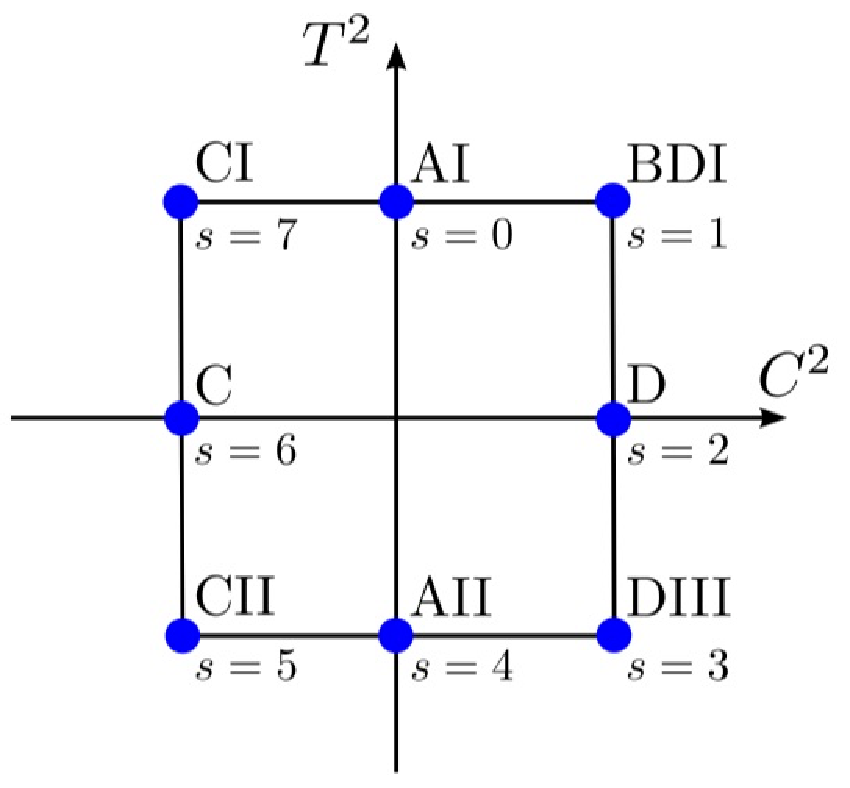
\includegraphics[width=.5\textwidth]{FigBottClock.pdf}
    \caption{关于时间反演对称性(T)和粒子-空穴对称性(C)的8个实对称群组成的8小时钟,被称为Bott钟。}
    \label{bottclock}
\end{figure}

\subsection{拓扑不变量}

以下我们讨论十重分类表\ref{tab:tenfoldway}里的体拓扑数,结论总结在表\ref{tab:ti}。这里讨论的拓扑不变量都是用Bloch-BdG哈密顿量的本征函数表示的。令第$a$个本征函数为$\ket{u^a(\vb k)}$,本征能量为$\varepsilon^a(\vb k)$,即$H(\vb k)\ket{u^a(\vb k)}=\varepsilon^a(\vb k) \ket{u^a(\vb k)}$。我们假设有能隙,费米能上下有$N_{+/-}$个能带,所以总能带是$N_-+N_+$。令被填充的Bloch波函数集合为$\Bqty{\ket{u_-^\alpha(\vb k)}}$,或者简写为$\Bqty{\ket{u^\alpha(\vb k)}}$,其中$\alpha=1,\dots,N_-$只标记被占据的能带。我们紧致化k空间到一个球:
\begin{equation}
  \vb k\in \text{BZ}^d\overset{\text{compactify}}{\longrightarrow}\mathrm{S}^d
\end{equation}
\subsubsection{$s$是偶数的主要系列:Chern数}
对于非手征类(即$s$是偶数),这个$\mathbb Z$类的拓扑是由陈数描述的
\begin{equation}
  c_n = \frac{1}{n!} \pqty{\frac{\iu}{2\pi}}^n \int_\bzd \Tr f^n
\end{equation}
其中$n=d/2$(注意这里暗示了Chern数只在偶数维是有良好定义)。Berry曲率是
\begin{equation}
  f=\dif a + a^2
\end{equation}
其中非阿贝尔Berry联络是
\begin{equation}
    a^{\alpha\beta}(\vb k) =\braket{u^\alpha(\vb k)}{\dif u^\beta(\vb k)}= \braket{u^\alpha(\vb k)}{\nabla_k u^\beta(\vb k)}\cdot \dif k.
\end{equation}
注意当系统有$\hat T$($\hat C$)时,在维度$d$满足$d\mod 4=2$(0)时,Chern数为零。而且在$s-d\mod 8=4$时,它一定是偶数。

陈数探测在底空间$\bzd$上光滑定义Bloch函数是否遇到阻碍。在给定$k$,基态是商空间$\mathrm{U}(N_++N_-)/\mathrm{U}(N_-)\times \mathrm{U}(N_+)$(被称为复的Grassmannian)的一个元素。Fermi-Dirac海可以用谱投影算符表示
\begin{equation}
  P(\vb k) = \sum_{\alpha=1}^{N_-} \ketbra{u^\alpha(\vb k)}{u^\alpha(\vb k)}\in \frac{\mathrm{U}(N_++N_-)}{\mathrm{U}(N_-)\times \mathrm{U}(N_+)}
\end{equation}
它是规范不变的。我们还定义$Q$矩阵
\begin{equation}
  Q(\vb k) = I - 2P(\vb k).
\end{equation}
它是厄米的,同时和$H(\vb k)$有相同的本征函数,不过本征值是$\pm 1$,因为$Q^2=1$。

波函数定义了一个纤维丛。注意到这些Bloch函数定义了一个从底空间到$\mathrm{U}(N_++N_-)/\mathrm{U}(N_-)\times \mathrm{U}(N_+)$的映射。拓扑不同的映射被同伦群描述
\begin{equation}
  \pi_d [\mathrm{U}(N_++N_-)/\mathrm{U}(N_-)\times \mathrm{U}(N_+)].
\end{equation}
对于足够大的$N_\pm$和偶数$d$,上式等于$\mathbb Z$。拓扑不同的映射被一个整数拓扑不变量描述
\begin{equation}
  \frac{-1}{2^{2n+1}}\frac{1}{n!}\Bqty{\frac{\iu}{2\pi}}^n\int_\bzd \Tr[Q(\dif Q)^{2n}].
\end{equation}
这即是Chern数。

\subsubsection{$s$是奇数的主要系列:缠绕数}
缠绕拓扑不变量$\nu$只能在有手征对称性时定义。为了简便,以下我们考虑$\Tr U_S=0$,即$N_+=N_-=N$的情况。这时谱投影算符不是复的Grassmannian的元素,而是$\mathrm{U}(N)$的元素。这可以由反块对角的哈密顿量看出
\begin{equation}
  H(\vb k) = \begin{bmatrix}
      0 & D(\vb k)\\
      D^\dagger(\vb k) & 0
  \end{bmatrix}\label{hkchiral}
\end{equation}
这时$Q$矩阵也是反块对角
\begin{equation}
  Q(\vb k) = \begin{bmatrix}
      0 & q(\vb k) \\
      q^\dagger(\vb k) & 0
  \end{bmatrix}
\end{equation}
其中$q(\vb k)$是一个幺正矩阵。所以$q$矩阵定义了一个从底空间$\bzd$到$\mathrm{U}(N)$的映射,拓扑不同的映射被同伦群$\pi_d [\mathrm{U}(N)]$描述。当$d$是奇数,$N$足够大时,$\pi_d[\mathrm{U}(N)]=\mathbb Z$。拓扑不同的映射被缠绕数表征
\begin{subequations}
    \begin{align}
        \nu_{2n+1}[q] &= \int_\bzd \omega_{2n+1}[q],\\
        \omega_{2n+1}[q] &= \frac{(-1)^n n!}{(2n+1)!}\bqty{\frac{\iu}{2\pi}}^{n+1}\Tr(q\inv \dif q)^{2n+1},
    \end{align}
\end{subequations}
其中$d=2n+1$是一个奇数。例如,在一维和三维,有
\begin{subequations}
    \begin{align}
        \nu_1 &=\frac{\iu}{2\pi}\int_{\text{BZ}} \Tr(q\inv\partial_k q)\dif k\\
    \nu_3 &= \frac{1}{24\pi^2}\int_{\text{BZ}} \epsilon^{\mu\nu\rho} \Tr\bqty{(q\inv\partial_\mu q)(q\inv\partial_\nu q)(q\inv\partial_\rho q)}
    \end{align}
\end{subequations}

Chern-Simons不变量也是定义在奇数维的,并且一般不是量子化的。但在有手征对称性是,它是量子化的。在$d=2n+1$维的Chern-Simons形式$y_{2n+1}$被定义为
\begin{equation}
  y_{2n+1}(a) = \frac{1}{n!}\pqty{\frac{\iu}{2\pi}}^{n+1}\int_0^1 \Tr(a f_t^n) \dif t
\end{equation}
其中
\begin{equation}
  f_t = t\dif a +t^2 a^2 = tf+(t^2-t)a^2.
\end{equation}
Chern-Simons形式在底空间的积分就是Chern-Simons不变量
\begin{equation}
  Y_{2n+1}[a] := \int_\bzd y_{2n+1}(a).
\end{equation}
例如,在$n=0,1$时,分别有
\begin{align}
  y_1(a) &= \frac{\iu}{2\pi}\Tr a,\\
  y_3(a) &= \frac{-1}{8\pi^2}\Tr \bqty{a\dif a+\frac{2}{3}a^3}
\end{align}
注意Chern-Simons形式和Chern-Simons不变量都不是规范不变的。但是对于两个不同的规范,
\begin{equation}
  a^g := g\inv a g + g\inv \dif g,\quad f^g = g\inv f g,\label{defagaugetransf}
\end{equation}
Chern-Simons形式的差和缠绕数密度只相差一个全微分
\begin{equation}
  y_{2n+1}(a^g) - y_{2n+1}(a) = \omega_{2n+1}[g] + \dif \alpha_{2n+1}(a,g).\label{difyomega}
\end{equation}
所以Chern-Simons形式在底空间的积分给出
\begin{equation}
  Y_{2n+1}(a^g)-Y_{2n+1}(a) \in \mathbb Z
\end{equation}
于是有
\begin{equation}
  W_{2n+1}:= \eu^{2\pi \iu Y_{2n+1}[a]}
\end{equation}
是良好定义、规范不变的量,虽然它不一定是量子化的。

上面的讨论都还是一般性地,现在我们考虑系统有手征对称性的情况。注意到式\eqref{hkchiral}对应的本征函数可直接写出
\begin{equation}
  \ket{u_\epsilon^\alpha(\vb k)}_N=\frac{1}{\sqrt{2}}\begin{bmatrix}
      \ket{n^\alpha}\\
      \epsilon q^\dagger(\vb k) \ket{n^\alpha}
  \end{bmatrix},\quad \epsilon=\pm.
\end{equation}
其中$\ket{n^\alpha}$是$N$个动量无关的正交归一向量。我们取$(n^\alpha)_\beta=\delta_{\alpha\beta}$。那么对应的Berry联络是$a_N=(1/2)q(\vb k)\dif q^\dagger(\vb k)$。注意到这个规范下,有$y_{2n+1}(a_N)=\omega_{2n+1}[q^\dagger]/2$。所以$Y_{2n+1}[a_N]=\nu_{2n+1}[q^\dagger]/2$,以及
\begin{equation}
  W_{2n+1} = \eu^{\pi \iu \nu_{2n+1}[q]}=\pm 1.
\end{equation}
也即,当有手征对称性时,$W_{2n+1}$只能取$\pm1$。比如当$d=1$($n=0$)时,Chern-Simons不变量$W_1$是定义在$\text{BZ}^{d=1}\simeq \mathrm{S}^1$上的$\mathrm{U}(1)$Wilson环。它的对数给出电极化,被手征对称性或者空间反演对称性量子化。这里$Y_1[a]$的非不变性对应于电子坐标位移在周期势中的定义只在一个晶胞内有意义,两个相差整数个晶格常数的位移是一样的。当$d=3$($n=1$)时,$Y_3$是量子化的磁电极化(或者被称为“$\theta$角”),
\begin{equation}
  \theta = 2 \pi \int_{\text{BZ}^3} y_3 \mod 2 \pi.
\end{equation}
它以轴子项的形式$\delta S=(\theta \alpha/4\pi)\int \vb E\cdot \vb B\dif^3\vb r$出现在电磁有效作用量里,其中$\alpha$是精细结构常数。这个量子化的磁电极化首先在三维时间反演对称的拓扑绝缘体中被提出。其实手征对称性和空间反演对称性也能量子化$W_3$。

\begin{table}[htb]
    \centering\small
    \caption{拓扑不变量。其中$\mathbb Z$不变量同时应用于复的和实的AZ类}
    \label{tab:ti}
    $$
    \begin{array}{l|cc}
        & \text{非手征类 ($s$是偶数} & \text{手征类($s$是奇数)}\\
        \hline
        \mathbb Z & \text{Chern数} & \text{缠绕数}\\
        \mathbb Z^{(1)}_2 & \text{Chern-Simons不变量} & \text{Fu-Kane不变量}\\
        \mathbb Z^{(2)}_2 & \text{Fu-Kane不变量} & \text{Chern-Simons不变量}
    \end{array}
    $$
\end{table}

\subsubsection{$s$是偶数的$\mathbb Z_2$第一后代}
对于上述讨论的主要系列,其体拓扑数是整数取值的Chern数。接下来讨论的第一和第二后代,其体拓扑数是$\mathbb Z_2$不变量。下面我们用两种策略讨论:首先从Chern-Simons不变量出发,利用对称性限制它可能的取值;其次我们也用陈数和Chern-Simons积分来构造$\mathbb Z_2$不变量。

第一$\mathbb Z_2$后代对应的拓扑不变量是
\begin{equation}
  Y_{2n-1} = \int_\bzd y_{2n-1} \in \frac{1}{2}\mathbb Z,\label{csiy}
\end{equation}
这里$n=(d+1)/2$。Chern-Simons不变量的定义可以相差任意整数。当有反幺正对称性时,Chern-Simons不变量只能取$1/2$的整数倍。当取到整数时$\mathbb Z_2$拓扑是平庸,当取到半整数时,它是拓扑非平庸的。

\paragraph{一维D类}
考虑一个在D类的一维BdG哈密顿量,它满足粒子-空穴对称性$C\inv H(-k) C= -H(k)$,其中$C=\tau_1 K$。类似于手征对称性,粒子-空穴对称性同样量子化$W=\eu^{2\pi \iu Y_1[a]}$到$\pm1$。回忆如果$\ket{u_-^\alpha(k)}$是一个负能量本征态,对应的本征能量是$-\varepsilon(k)$,那么$\ket{\tau_1 u_-^{*\alpha}(-k)}$是一个正能量本征态,对应的本征能量是$\varepsilon(k)$。所以负能量本征态和正能量本征态的Berry联络是关联的
\begin{equation}
  A_-^{\alpha\beta} (k) = \braket{u_-^\alpha(k)}{\partial_k u_-^\beta(k)}=A_+^{\alpha\beta}(-k).
\end{equation}
因此一维Chern-Simons积分是
\begin{align}
  \int_{-\pi}^{+\pi} \Tr A_- \dif k &= \int_0^\pi \Tr[A_- +A_+]\dif k\nonumber\\
  &= \int_0^\pi u_i^{* a}\partial_k u_i^a \dif k = \int_0^\pi \Tr U^\dagger\partial_k U \dif k,
\end{align}
其中$a$取到所有能带,$\alpha$只取一半能带(即负能带)。这里幺正矩阵$U$被定义为$U_i^a(k) = u_i^a(k)$。注意到$\int_0^\pi \Tr U^\dagger \partial_k U\dif k= \int_0^\pi \partial_k \ln\det[U(k)]\dif k=\ln\det U(\pi) - \ln\det U(0)$,这个Chern-Simons不变量变成
\begin{equation}
  W_1=\eu^{2\pi \iu Y_1 }=[\det[U(\pi)]\inv[\det U(0)].\label{w1detu}
\end{equation}
在粒子-空穴不变动量处$k=0,\pi$,幺正矩阵$U(k)$有特殊性质,上式可以进一步简化。下面我们先回顾BdG哈密顿量的一般性质(一个更一般地、统一了费米子和玻色子的讨论在下一章给出)再给出$W$的简化表达式。定义Nambu旋量
\begin{subequations}
    \begin{align}
  \Gamma = \begin{bmatrix}
      c_1 & \cdots & c_N & c_1^\dagger & \cdots c_N^\dagger
  \end{bmatrix}^T,\\
  \Gamma^\dagger = \begin{bmatrix}
      c_1^\dagger & \cdots & c_N^\dagger & c_1 & \cdots c_N
  \end{bmatrix}.
\end{align}
\end{subequations}
它们满足正则反对易关系$\Bqty{\Gamma_A,\Gamma^\dagger_B}=\delta_{AB}$($A,B=1,\dots,2N$)。注意它们不是独立的
\begin{equation}
  (\tau_1 \Gamma)^T = \Gamma^\dagger ,\quad (\Gamma^\dagger \tau_1)^T = \Gamma.\label{gammarelation}
\end{equation}
其中$\tau_1$作用在Nambu空间。利用这个Nambu旋量,BdG哈密顿量$\hat H$被写成
\begin{equation}
  \hat H = \frac{1}{2}\Gamma^\dagger H \Gamma.
\end{equation}
由于式\eqref{gammarelation},单粒子哈密顿量满足粒子-空穴对称性,
\begin{equation}
  \hat H = \frac{1}{2}(\tau_1\Gamma)^T H (\Gamma^\dagger \tau_1)^T = -\frac{1}{2}\Gamma^\dagger(\tau_1 H\tau_1)^T \Gamma + \frac{1}{2}\Tr(\tau_1 H\tau_1).
\end{equation}
即
\begin{equation}
  \tau_1 H^T \tau_1 = -H \Leftrightarrow \tau_1 H^* \tau_1 = -H.
\end{equation}
由于上式,任意一个BdG哈密顿量总可以写成
\begin{equation}
  H= \begin{bmatrix}
      \Xi & \Delta\\
      -\Delta^* & -\Xi^T
  \end{bmatrix},\quad \Xi = \Xi^\dagger ,\quad \Delta =- \Delta^T,
\end{equation}
其中$\Xi$被称为“正常”部分,$\Delta$被称为“反常”部分(即配对项)。这个BdG哈密顿量可以被看成Majorana费米子的单粒子哈密顿量,
\begin{equation}
  \begin{bmatrix}
      \lambda_I\\
      \lambda_{I+N}
  \end{bmatrix}=\begin{bmatrix}
      c_I + c_I^\dagger \\
      \iu (c_I - c_I^\dagger)
  \end{bmatrix},\label{majoranadef}
\end{equation}
其中Majorana费米子满足
\begin{equation}
  \Bqty{\lambda_A,\lambda_B} = 2\delta_{AB},\quad \lambda_A^\dagger = \lambda_A\quad (A,B=1,\dots,2N).
\end{equation}
注意式\eqref{majoranadef}实际上是一个Cayley变换,$\lambda = T_{\text{Cayley}} \Gamma$,这里
\begin{equation}
  T_{\text{Cayley}} = \begin{bmatrix}
      I_N & I_N\\
      \iu I_N & -\iu I_N
  \end{bmatrix}.
\end{equation}
在这个Majorana基下,BdG哈密顿量可以被写成
\begin{equation}
  \hat H = \iu \lambda X \lambda,\quad X^* = X,\quad X^T = -X
\end{equation}
这里的$2N\times 2N$矩阵$X$可以用$\Xi$和$\Delta$表示
\begin{equation}
  \iu X = \frac{1}{8}\begin{bmatrix}
      R_- + S_- & -\iu (R_+ -S_+)\\
      \iu (R_+ +S_+) & R_- -S_-
  \end{bmatrix},
\end{equation}
其中
\begin{equation}
  R_\pm =\Xi \pm \Xi^T = \pm R_\pm^T ,\quad S_\pm = \Delta\pm \Delta^* =-S_\pm^T.
\end{equation}
注意到对于任意一个实的反对称矩阵,例如这里的$X$,我们总可以通过一个正交变换把它写成块对角的形式
\begin{equation}
  X= O\Sigma O^T,\quad \Sigma = \begin{bmatrix}
      0 & \varepsilon_1 & & &\\
      -\varepsilon_1 & 0 & & &\\
      & & \ddots & & \\
      & & & 0 & \varepsilon_N\\
      & & & -\varepsilon_N & 0
  \end{bmatrix}\label{xdef}
\end{equation}
其中$O$是正交的,且有$\varepsilon_l\geq 0$。在旋转后的基$\xi:= O^T\lambda $下,哈密顿量变成$\hat H = \iu \xi^T \Sigma \xi = 2 \sum_{I=1}^N \varepsilon_I \xi_{2I-1} \xi_{2I}$。回到式\eqref{w1detu},利用Majorana基,我们把$H(k)$写成$X(k)$。由于在时间反演不变动量处有$\tau_1 H^*(k) \tau_1 = -H(k)$,所以$X(k=0,\pi)$是实的反对称矩阵。通过一个正交矩阵$O(k=0,\pi)$,我们可以把它写成如式\eqref{xdef}那样的正则形式。于是$W$可以用$O(k=0,\pi)$写出
\begin{equation}
  W= [\det O(\pi)]\inv [\det O(0)].
\end{equation}
由于$O(k=0,\pi)$是正交矩阵,它们的行列式是$\pm1$,所以$W=\pm1$。利用一个$2n$维反对称矩阵的Pfaffian,
\begin{equation}
  \pf(X) = \frac{1}{2^n n!} \sum_{\sigma\in \mathrm{S}_{2n}} (-1)^{\abs{\sigma}} X_{\sigma(1)\sigma(2)}\cdots X_{\sigma(2n-1)\sigma(2n)},
\end{equation}
并且注意到$\pf(OXO^T)= \pf(X)\det O$和$\sgn(\pf[X(k)]\det O(k))=1$,所以$W$也可以写成
\begin{equation}
  W=\sgn (\pf[X(0)]\pf[X(\pi)]),
\end{equation}
它是明显规范不变的。

\paragraph{三维AII类}
下面我们讨论三维时间反演对称的拓扑绝缘体,其拓扑性质是由时间反演对称性保护的,$T\inv H(-k) T = H(k)$。由于这个关系,Bloch波函数在$\vb k$和$-\vb k$是联系的。如果$\ket{u^\alpha(\vb k)}$是在$\vb k$处的一个本征态,那么$T\ket{u^\alpha(\vb k)}$是在$-\vb k$处的一个本征态。假设我们在整个BZ光滑定义$\ket{u^\alpha(\vb k)}$。(由于时间反演对称性,陈数为零,所以这总是可以的。)我们可以比较$\ket{u^\alpha(-\vb k)}$和$T\ket{u^\alpha(\vb k)}$。它们一定是通过一个幺正矩阵联系$\ket{u^\alpha(-\vb k)}=[w^{\alpha\beta}(\vb k)]^*\ket{Tu^\beta(\vb k)}$。所以我们定义缝合矩阵
\begin{equation}
  w^{\alpha\beta}(\vb k) = \braket{u^\alpha(-\vb k)}{Tu^\beta(\vb k)}.
\end{equation}
它是在$-\vb k$的被占据的本征态和在$\vb k$的被占据的本征态的时间反演的像的交叠。注意这个矩阵满足(因为$T$是反线性和反幺正的,且$T^2=-1$)
\begin{equation}
  w^{\alpha\beta}(-\vb k)= -w^{\alpha\beta}(\vb k).
\end{equation}
因此Berry联络在$\vb k$和$-\vb k$处是关联的
\begin{equation}
  A_\mu(-\vb k) = - w(\vb k) A_\mu^*(\vb k) w^\dagger(\vb k) - w(\vb k)\partial_\mu w^\dagger(\vb k).\label{akamk}
\end{equation}
即$-A_\mu (-\vb k)$和$A_\mu^*(\vb k) = -A^T_\mu (\vb k)$是通过一个规范变换联系的。下面我们证明Chern-Simons不变量是缝合矩阵$w$的缠绕数,
\begin{equation}
  Y[a] = \frac{1}{2}\int_{\text{BZ}} \omega[w] = \frac{1}{2} \times \mathbb Z\label{yawinding}
\end{equation}
也即$W=\eu^{2\pi \iu Y[a]} = \pm 1$。在积分$Y[a]$中做变量代换$\vb k\rightarrow -\vb k$,再利用式\eqref{akamk}和定义式\eqref{defagaugetransf},$A_\mu (-\vb k) = -[A^{g^*}_\mu(\vb k)]^*$,其中$g=w^\dagger$,我们有$Y[a]=-Y[(a^{g^*})^*]=-(Y[a^{g^*}])^*=-Y[a^{g^*}]$,这里最后一个等式用到了$Y[a]$是实数的性质。最后我们利用式\eqref{difyomega},
\begin{equation}
  Y[a]=-Y[a]-\int_{\text{BZ}} \Bqty{\omega[g^*] + \dif \alpha (a,g^*)}
\end{equation}
和$\int_{\text{BZ}}\omega[g]= \int_{\text{BZ}}\omega[w^\dagger] = -\int_{\text{BZ}} \omega[w]$即得到式\eqref{yawinding}。这个Chern-Simons不变量也可以用缝合函数$w$在在时间反演不变动量$K$处的Pfaffian表示
\begin{equation}
  W= \prod_{K} \frac{\pf[w(K)]}{\sqrt{\det[w(K)]}}.\label{pfdefz2}
\end{equation}

\subsubsection{$s$是偶数的$\mathbb Z_2$第二后代}
应用于$s$是偶数(即非手征对称类)的$\mathbb Z_2$第二后代的拓扑不变量定义为
\begin{equation}
  \mathrm{FK}_n = \frac{1}{n!}\bqty{\frac{\iu}{2\pi}}^2\int_{\bzd_{1/2}}\Tr(f^n) - \oint_{\partial \bzd_{1/2}} y_{2n-1}\label{deffk}
\end{equation}
其中$n=d/2$。这个积分的第一项是在BZ的一半空间上进行的,比如取$k_1\in[0,\pi]$。我们要求这一半空间和它在第一BZ的补集有时间反演关系。第二项的Chern-Simons积分是在这个一半空间的边界上进行的。这个边界是规范相关的,需要特别小心选取基矢。对于时间反演不变的系统,我们要求规范限制
\begin{equation}
  w^{\alpha\beta}(\vb k) = \braket{u^\alpha(-\vb k)}{Tu^\beta(\vb k)}=\text{const},\label{gaugeconstraint1}
\end{equation}
对于$\vb k\in \partial\bzd_{1/2}$。例如对于二维AII类的拓扑绝缘体,FK不变量要求$w(\vb k)=\iu \sigma_2$。对于有粒子-空穴对称性的系统(D类和C类),一个占据态$\ket{u^\alpha(\vb k)}$在粒子-空穴算符$C$的作用下变成一个非占据态$\ket{v^\alpha(\vb k)}=\ket{Cu^\alpha(-\vb k)}$,式\eqref{deffk}中的Chern-Simons形式对占据态有如下要求
\begin{equation}
  \int_{\partial\bzd_{1/2}}\Tr [(X\dif X^\dagger)^{d-1}]=0,\label{gaugeconstraint2}
\end{equation}
其中$X(\vb k)=\begin{bmatrix}
    u^1 & \dots & u^N & v^1 & \dots & v^N
\end{bmatrix}$
是一个由本征态构成的幺正矩阵。上述两个规范限制是必须的。不然Chern-Simons积分可以在一个大规范变换下相差任意整数。这些条件使FK不变量只能取$\mathbb Z_2 = \Bqty{0,1}$。

\paragraph{二维AII类}

二维时间反演对称的拓扑绝缘体的体拓扑数由式\eqref{deffk}给出。类似于三维时间反演对称拓扑绝缘体,我们也可以用式\eqref{pfdefz2}。事实上我们还可以用时间反演不变极化\cite{Fu2006}和Wilson环\cite{Yu2011}来表示。

\subsubsection{$s$是奇数的$\mathbb Z_2$第一后代}
属于手征类的第一$\mathbb Z_2$后代和属于非手征类的第二$\mathbb Z_2$后代有同构关系。所以前者的体拓扑数和后者一样,即FK不变量,式\eqref{deffk}。注意对于$s=1,5$(即CI类和DIII类),我们仍需要规范限制,式\eqref{gaugeconstraint1};对于$s=3,7$(即BDI类和CII类),我们仍需要规范限制,式\eqref{gaugeconstraint2}。

\paragraph{二维DIII类}
类似于二维时间反演对称的拓扑绝缘体(AII类),二维的时间反演对称的拓扑超导体的FK不变量也可以写出式\eqref{pfdefz2}。这个Pfaffian公式也可以用$Q$矩阵写出。我们首先把BdG哈密顿量写出块反对角的形式
\begin{equation}
  H(\vb k) = \begin{bmatrix}
      0 & D(\vb k) \\
      D^\dagger(\vb k) & 0
  \end{bmatrix},\quad D(\vb k) = -D^T(-\vb k).
\end{equation}
在这个表象下,时间反演算符是$T=U_TK=\iu \sigma_2 \otimes I K$,而$Q$矩阵是
\begin{equation}
  Q(\vb k) = \begin{bmatrix}
      0 & q(\vb k) \\
      q^\dagger(\vb k) & 0
  \end{bmatrix},\quad q(\vb k) = -q^T(-\vb k).
\end{equation}
这个基下缝合矩阵是$w^{\alpha\beta}(\vb k) = -q^{\alpha\beta}(-\vb k)$。所以$\mathbb Z_2$拓扑不变量是
\begin{equation}
  W=\prod_K \frac{\pf[q(K)]}{\sqrt{\det [q(K)]}}
\end{equation}
其中$K$是二维BZ里的时间反演不变动量。

\subsubsection{$s$是奇数的$\mathbb Z_2$第二后代}

手征类的第二$\mathbb Z_2$后代的体拓扑数是由式\eqref{csiy}给出的Chern-Simons不变量$Y_{2n-1}$,其中$n=(d+1)/2$。类似于FK不变量,这里的被占据态需要满足规范限制,对于CI类和DIII类,它是式\eqref{gaugeconstraint1};对于BDI类和CII类,它是式\eqref{gaugeconstraint2}。由于反幺正对称性,这些规范限制使Chern-Simons不变量是整数。$\mathbb Z_2$拓扑是平凡的如果$Y_{2n-1}$是偶数,反之是非平凡的。

\paragraph{一维DIII类}
在一维,规范限制\eqref{gaugeconstraint1}是自动满足的。式\eqref{csiy}变成了“极化”,它是整数取值的。通过取基使哈密顿量和$Q$矩阵变成块反对角的,这个Chern-Simons不变量化简为以下的$\mathbb Z_2$不变量
\begin{equation}
  (-1)^\nu = \frac{\pf[q(\pi)]}{\pf[q(0)]}\frac{\sqrt{\det[q(0)]}}{\sqrt{\det[q(\pi)]}}.
\end{equation}

\subsection{拓扑边缘态和体边对应关系}
\label{subsec:tebbc}
所谓的体边对应关系,就是指系统取周期边界条件时的体拓扑不变量和取开放边界条件时局域在边缘的拓扑保护零能模有一一对应关系。数学上,这个关系与Atiyah-Singer指标定理有密切联系,具体的讨论涉及到代数K理论、椭圆微分算子理论等,详见\cite{Chiu2016}以及那里提到的文献。物理上,这个现象是容易理解的:根据定义,拓扑非平庸和平庸的态在相图上总是由一个量子相变分开的。这个事实暗示了当一个拓扑绝缘体或拓扑超导体靠近一个拓扑平庸相时,两相的交界处一定会有零能态。这个零能(临界)态的出现可以被认为是由于发生了一个在空间局域的相变,在那里哈密顿量的参数沿着边界的横向改变。注意到只要给定的微扰不破坏体能隙和系统对称性,对应的零能边界态就总是存在的,在这个意义上我们说零能边界态是拓扑保护的。特别地,这些无能隙边界态是对无序完全免疫的,而且也不会发生Anderson局域化。这些无能隙边界态是拓扑绝缘体和拓扑超导体最重要的特征,事实上它们可以被用来作为后者的定义。











